% Chapter 07 - Acid-Base Equilibrium.tex
% Copyright (c) 2014 - 2016, zhiayang@gmail.com
% Licensed under the Apache License Version 2.0.


\pagebreak
\part{Acid-Base Equilibrium}

	\section{Theory of Acids and Bases}

		\subsection{Brønsted-Lowry}

			Fundamental to understanding this chapter is the Brønsted-Lowry theory of acids and bases... as the section header would lead you
			to conclude.

			\begin{bulletlist}
				& Brønsted acids \itl{donate} a proton (\ch{H+}) to a base
				& Brønsted bases correspondingly \itl{accept} a proton (\ch{H+}) from an acid.
			\end{bulletlist}

			Thus, there are some restrictions placed on each --- acids must contain one or more atoms of \ch{H} to donate, and bases must have
			one or more lone pairs in order to accept the \ch{H+} ion.

			As such, acid-base reactions in the context of this theory involves the transfer of a proton from a Brønsted acid to a Brønsted base.

			Note that, in the context of aqueous reactions, \ch{H+} can also be represented by \ch{H3O+}, which is probably how it exists IRL.

		% end subsection

		\subsection{Lewis}

			While Brønsted acids and bases are defined in terms of the transfer of protons, Lewis acids and bases are defined in terms of the
			transfer of electron pairs. Thus:

			\begin{bulletlist}
				& Lewis acids \itl{accept} an electron pair from a Lewis base donor.
				& Lewis bases correspondingly \itl{donate} an electron pair to a Lewis acid.
			\end{bulletlist}

			Further references to acids or bases implicitly refer to the \itl{Brønsted} definition.

		% subsection



		\pagebreak
		\subsection{Conjugate Acid-Base Pairs}

			When a acid loses the \ch{H+} ion, an anion is naturally left --- this is the conjugate base of the acid. Conversely, when a
			base accepts a proton, it forms the conjugate acid of the base.

			\txtdiagram{
				\schemestart[0,1.0,thick]
					\chemname{\ch{CH3CO2H}}{\tinytext{acid}}\hspace{7mm} + \hspace{7mm}\chemname{\ch{NH3}}{\tinytext{base}}
					\arrow(.mid east--.mid west){<=>}
					\chemname{\ch{CH3CO2-}}{\tinytext{conjugate base}}\hspace{7mm} + \hspace{7mm}\chemname{\ch{NH4+}}{\tinytext{conjugate acid}}
				\schemestop
			}{\vspace{-1.5em}}

			It should be immediately clear that this is an \itl{equilibrium} reaction.

			In the forward reaction, \ch{CH3CO2H} acts as the acid, donating a proton to the base, \ch{NH3}. In the reverse direction,
			\ch{NH4+} is the acid, donating a proton to the base \ch{CH3CO2-}.

			 Furthermore, \ch{CH3CO2H} and \ch{CH3CO2-} are \itl{conjugate pairs}, as are \ch{NH3} and \ch{NH4+}. Conjugate pairs always
			 differ by a proton, and in any given acid-base reaction, there are two such pairs.

		% subsection


		\subsection{Strength of Acids and Bases}

			It is important to note that the \itl{strength} of an acid or base is distinct from its \itl{concentration} in solution;
			it is possible to have a strong, dilute acid, or a weak, concentrated base.

			\subsubsection{Strong Acids and Bases}

				The strength of an acid or base is given as the degree of dissociation from the acid or base into ions, in solution. A strong
				acid or base is one that ionises \itl{completely} in solution to give \ch{H+} or \ch{OH-} respectively.

				\txtdiagram{
					\schemestart[0,1.0,thick]
						\chemname{\ch{H\Cl}}{\tinytext{strong acid}}\hspace{7mm} + \hspace{7mm}\chemname{\ch{H2O}}{}
						\arrow(.mid east--.mid west){->}
						\chemname{\ch{\Cl-}}{\tinytext{weak conjugate base}}\hspace{7mm} + \hspace{7mm}\chemname{\ch{H3O+}}{}
						\arrow(@c1.south east--.north east){0}[-90,.5]
						\chemname{\ch{NaOH}}{\tinytext{strong base}}
						\arrow(.mid east--.mid west){->}
						\chemname{\ch{OH-}}{}\hspace{7mm} + \hspace{7mm}\chemname{\ch{Na+}}{}
					\schemestop
				}{\vspace{-1.5em}}

				Since they ionise \itl{completely}, the reverse reaction is negligible, so the reaction is written with a single-headed
				arrow, \ch{->}. This is because the conjugate base \ch{\Cl-}, in the case of \ch{H\Cl}, has a low tendency to
				accept a proton.

			% end subsubsection


			\pagebreak
			\subsubsection{Weak Acids and Bases}

				Weak acids and bases, on the other hand, only dissociate \itl{partially} in water to give \ch{H+} and \ch{OH-}. Thus, they
				are in an equilibrium with their conjugate, so the reaction is written with a double-headed arrow, \ch{>=<}.

				\txtdiagram{
					\schemestart[0,1.0,thick]
						\chemname{\ch{CH3CO2H}}{\tinytext{weak acid}}\hspace{7mm} + \hspace{7mm}\chemname{\ch{H2O}}{}
						\arrow(.mid east--.mid west){<=>}
						\chemname{\ch{CH3CO2-}}{\tinytext{conjugate base}}\hspace{7mm} + \hspace{7mm}\chemname{\ch{H3O+}}{}
						\arrow(@c1.south east--.north east){0}[-90,.5]
						\chemname{\ch{NH3}}{\tinytext{weak base}}\hspace{7mm} + \hspace{7mm}\chemname{\ch{H2O}}{}
						\arrow(.mid east--.mid west){<=>}
						\chemname{\ch{NH4+}}{\tinytext{conjugate acid}}\hspace{7mm} + \hspace{7mm}\chemname{\ch{OH-}}{}
					\schemestop
				}{\vspace{-1.5em}}

				Since this is an equilibrium reaction, a mixture of the undissociated acid or base, as well as its dissociated ions,
				exist in solution.

			% end subsubsection

		% end subsection

	% end section

	\section{\MpH{}, \MpOH{} and Other Such Constants}

		First, the general idea of \itl{p} should be stated. In essence, it is this:

		\txtdiagram{
			$pX = -lg(X)$, \hspace{5mm} $X = 10^{-pX}$
		}{\vspace{-2em}}

		So, it follows \pH{} and \pOH{} are, respectively,

		\txtdiagram{
			$pH = -lg([H^{+}])$, \hspace{5mm} $[H^{+}] = 10^{-pH}$
			\linebreak
			\linebreak
			$pOH = -lg([OH^{-}])$, \hspace{5mm} $[OH^{-}] = 10^{-pOH}$
		}{\vspace{-2em}}

		In other words, it is a measure of the concentration of either \ch{H+} or \ch{OH-} in the solution. As you might be aware, the
		lower the \pH{}, the more \ch{H+} there is. \pOH{} is similar, although it obviously measures the concentration of \ch{OH-}.

		Note that neither \pH{} nor \pOH{} should be used to compare acid strengths --- as previously mentioned, strength is independent
		of concentration. It can only be used as a comparison when both acids have the same initial concentration.


		\pagebreak
		\subsection{Ionic Product of Water, \MKw{}}

			Pure water actually \itl{auto-ionises} to a very slight degree, giving \ch{H+ \stAq} and \ch{OH- \stAq}.

			\txtdiagram{
				\schemestart[0,1.0,thick]
					\ch{H2O \stL}\hspace{2mm} + \hspace{2mm}\ch{H2O \stL}
					\arrow{<=>}
					\ch{H3O+ \stAq}\hspace{2mm} + \hspace{2mm}\ch{OH- \stAq}
				\schemestop
			}{\vspace{-1.5em}}

			Since this is an equilibrium, the \Kc{} value is as such:

			\diagram[1.5]{
				$K_{c} = \frac{[H^{+}][OH^{-}]}{[H_{2}O]}$
			}{\vspace{-2em}}

			Given that the extent of ionisation is minuscule, the ``concentration'' of \ch{H2O} is almost constant, and so

			\txtdiagram{
				$K_{c} \times [H_{2}O] = [H^{+}][OH^{-}]$
				\linebreak
				\linebreak
				$K_{w} = K_{c} \times [H_{2}O] = [H^{+}][OH^{-}]$
			}{\vspace{-2em}}

			Thus, \pKw{} becomes relatively simple, taking $lg$ on both sides:

			\txtdiagram{
				$pK_{w} = pH + pOH$
			}{\vspace{-2em}}

			Experimentally, it is found that, at \SI{25}{\celsius}, $K_{w} = \SI{1.0e-14}{\molarConc}$, so:
			\begin{bulletlist}
				& $pK_{w} = 14$
				& $pH + pOH = 14$.
			\end{bulletlist}

			The value of \Kw{}, and by extension, \pKw{}, is affected solely by temperature, just like \Kc{}. Thus, only at \SI{25}{\celsius}
			does $pH + pOH = 14$ hold; at higher temperatures, \Kw{} \itl{increases}, so the sum is \itl{greater than} \num{14}.

			Of course, the relationships $pH + pOH = pK_{w}$ and $K_{w} = [H^{+}][OH^{-}]$ always hold.

		% end subsection


		\pagebreak
		\subsection{\MpH{} and \MpOH{} of Strong Acids and Bases}

			Given that strong acids and bases dissociated completely in water, [\ch{H+}] and [\ch{OH-}] simply become the initial concentration
			of the corresponding acid or base. If the acid in question is di- or even tri-protic, then the concentration of \ch{H+} will need
			to be multiplied by the appropriate ratio --- the same applies for bases, of course.

			There is an edge case if the initial concentration of the strong acid or base is smaller than \SI{1.0e-7}{\molarConc}; in this case,
			the molecules of \ch{H+} or \ch{OH-} from the auto-ionisation of water must be taken into account --- it is as simple as adding
			\num{1.0e-7} to the concentration of the acid or base.

		% end subsection

	% end section



	\pagebreak
	\section{Dissociation of Acids and Bases}

		The acid and base dissociation constants, \Ka{} and \Kb{} respectively, are indicators of the degree of dissociation of the given acid
		or base.

		Additionally, given the definitions of both \Ka{} and \Kb{}, the following relationships hold, for a given
		\itl{conjugate acid-base pair}. Naturally it doesn't make sense to compare or relate two unrelated species.

		\txtdiagram{
			$K_{a} \times K_{b} = K_{w}$
			\linebreak
			\linebreak
			$pK_{a} + pK_{b} = pK_{w}$
		}{\vspace{-2em}}

		Thus, the weaker the acid, the stronger its conjugate base, and vice-versa.


		\subsection{Acid Dissociation Constant, \MKa{}}

			For some general weak acid \ch{HA}, it dissociates partially in water:

			\txtdiagram{
				\schemestart[0,1.0,thick]
					\ch{HA \stAq}\hspace{2mm} + \hspace{2mm}\ch{H2O \stL}
					\arrow{<=>}
					\ch{H3O+ \stAq}\hspace{2mm} + \hspace{2mm}\ch{A- \stAq}
				\schemestop
			}{\vspace{-1.5em}}

			In a dilute solution, [\ch{H2O}] is almost constant, so the equilibrium constant can be defined as such:

			\diagram[1.5]{
				$K_{a} = \frac{[H^{+}][A^{-}]}{[HA]}$
			}{\vspace{-2em}}

			Naturally this is only true when the system is at equilibrium. Thus, the acid dissociation constant \Ka{} is simply the
			equilibrium constant for the dissociation equilibrium, and indicates the \itl{extent} to which the acid dissociates.

			Additionally, \pKa{} is defined similarly to \pKw{}:

			\txtdiagram{
				$pK_{a} = -lg(K_{a})$
			}{\vspace{-2em}}

			The larger the value of \Ka{} (and conversely, the smaller the value of \pKa{}), the stronger the acid is. Thus, \Ka{}
			values should be used as the basis for comparing the strength of weak acids. Naturally, the \Ka{} values should be
			taken at the same temperature for a valid comparison.

			Note that the \Ka{} value for strong acids like \ch{H\Cl} is very large, and is often irrelevant.



		% end subsection


		\pagebreak
		\subsection{Base Dissociation Constant, \MKb{}}

			The definitions of \Kb{} and \pKb{} are essentially the mirror images of \Ka{} and \pKa{}. For a given weak base \ch{B}:

			\txtdiagram{
				\schemestart[0,1.0,thick]
					\ch{B \stAq}\hspace{2mm} + \hspace{2mm}\ch{H2O \stL}
					\arrow{<=>}
					\ch{BH+ \stAq}\hspace{2mm} + \hspace{2mm}\ch{OH- \stAq}
				\schemestop
			}{\vspace{-1.5em}}

			Thus, the base dissociation constant \Kb{} can be defined:

			\diagram[1.5]{
				$K_{b} = \frac{[BH^{+}][OH^{-}]}{[B]}$
			}{\vspace{-2em}}

			\pKb{} can also be defined similarly:

			\txtdiagram{
				$pK_{b} = -lg(K_{b})$
			}{\vspace{-2em}}

			As with acids, the larger the value of \Kb{}, the stronger the base.

		% end subsection


		\subsection{Degree of Dissociation, \chemalpha}

			The degree of dissociation of a given acid or base is the \itl{ratio} of the number of moles of the substance that are ionised, to
			the number of unionised moles of acid or base.

			\diagram[1.5]{
				$\alpha = \frac{[acid]_{dissociated}}{[acid]_{initial}}$
			}{\vspace{-1.5em}}

			Thus, for a strong acid or base, α is close to \num{1}, while it is often much smaller than \num{1} for weak acids or bases.

		% end subsection


		\subsection{Calculations involving \MKa{} and \MKb{}}

			Calculations involving only \Ka{} or \Kb{} are fairly straightforward. Given the value of \Ka{} for instance, it is trivial
			to find the concentration of \ch{H+} and hence \pH{}, \itl{assuming}:

			\begin{bulletlist}
				& $[H^{+}] = [A^{-}]$, ie. all the \ch{H+} and \ch{A-} comes from the acid
				& $[HA]$ at equilibrium $ = [HA]$ initially
			\end{bulletlist}

			The first assumption will be \itl{invalid} when there are \itl{external sources} of \ch{H+} or \ch{A-}, as in a buffer
			system. The second assumption can be discarded to be more accurate, but should be used when $[H^{+}] << 0.1$.

		% end subsection

	% end section

	\pagebreak
	\section{Salt Hydrolysis}

		Two main categories of salts undergo hydrolysis in water, forming \ch{H3O+} and \ch{OH-} ions to give acidic or basic solutions
		respectively --- ions of salts derived from weak acids or bases, and metal cations with a high charge density.

		Ions of salts derived from strong acids and bases, eg. \ch{Na\Cl} or \ch{KNO3}, will not hydrolyse, and will give a neutral solution.


		\subsection{Weak Acid, Strong Base}

			Examples of such salts include \ch{CH3CO2- Na+}, which comes from the weak acid \ch{CH3CO2H} and the strong base \ch{NaOH}.
			The \ch{Na+} ion will not hydrolyse, while the \ch{CH3CO2-} ion will:

			\txtdiagram{
				\schemestart[0,1.0,thick]
					\chemname{\ch{CH3CO2- \stAq}}{\tinytext{stronger con-base}}\hspace{2mm} + \hspace{2mm}\chemname{\ch{H2O \stL}}{}
					\arrow(.mid east--.mid west){<=>}
					\chemname{\ch{CH3CO2H \stAq}}{\tinytext{weaker acid}}\hspace{2mm} + \hspace{2mm}\chemname{\ch{OH- \stAq}}{}
				\schemestop
			}{\vspace{-1.5em}}

			In this case, given that \ch{CH3CO2H} is a weaker acid than water, \ch{CH3CO2-} is a stronger base than water, thus it is
			able to accept a proton --- leaving \ch{CH3CO2H} and \ch{OH-} as the products.

			Since \ch{OH-} is present, the solution would be \itl{alkaline}. However, \ch{CH3CO2-} is still an objectively weak base
			(water is a low benchmark), so the system exists in an equilibrium.

		% end subsection


		\subsection{Strong Acid, Weak Base}
			\ch{NH4+ \Cl-}, which comes from the weak base \ch{NH3} and the strong acid \ch{H\Cl}, can have its \ch{NH4+} ion undergo
			salt hydrolysis as well, in what is basically the mirror of the case with a strong base and weak acid:

			\txtdiagram{
				\schemestart[0,1.0,thick]
					\chemname{\ch{NH4+ \stAq}}{\tinytext{stronger con-acid}}\hspace{2mm} + \hspace{2mm}\chemname{\ch{H2O \stL}}{}
					\arrow(.mid east--.mid west){<=>}
					\chemname{\ch{NH3 \stAq}}{\tinytext{weaker base}}\hspace{2mm} + \hspace{2mm}\chemname{\ch{H3O+ \stAq}}{}
				\schemestop
			}{\vspace{-1.5em}}

			Again, \ch{NH4+} is a stronger acid than water, given that \ch{NH3} is weaker than water. Hence it donates a proton to \ch{H2O},
			forming \ch{H3O+} and giving an \itl{acidic} solution.

			Also, this system also exists in an equilibrium.

		% end subsection


		\pagebreak
		\subsection{Weak Acid and Weak Base}

			In this case, such as with the salt \ch{CH3CO2- NH4+}, both ions will hydrolyse --- the final \pH{} of the solution depends on
			the \Ka{} and \Kb{} values of the conjugate acid and base respectively. Generally speaking, the cation is the conjugate acid,
			and the anion is the conjugate base.

			\begin{bulletlist}
				& $K_{a} > K_{b}$;\hspace{4mm} $[H_{3}O^{+}] > [OH^{-}]$;\hspace{4mm} acidic solution
				& $K_{a} = K_{b}$;\hspace{4mm} $[H_{3}O^{+}] = [OH^{-}]$;\hspace{4mm} neutral solution
				& $K_{a} < K_{b}$;\hspace{4mm} $[H_{3}O^{+}] < [OH^{-}]$;\hspace{4mm} basic solution
			\end{bulletlist}

		% end subsection


		\subsection{Metal Cation With High Charge Density}

			There are 3 main metal cations exhibiting this property --- \ch{\Al^3+}, \ch{Cr^3+}, and \ch{Fe^3+}. As will be covered later
			in the \itl{Chemistry of Transition Metals}, these ions can form complexes with \ch{H2O} ligands in aqueous solution.

			Due to their high charge density, they are able to sufficiently polarise and weaken an \ch{O-H} bond in one of the ligands,
			allowing an external \ch{H2O} molecule to gain a proton. This of course requires breaking said \ch{O-H} bond, hence hydrolysis.

			The \ch{H3O+} molecule is formed, so the solution becomes acidic.


			\txtdiagram{
				\schemestart[0,1.0,thick]
					\ch{[\Al(H2O)6]^3+ \stAq}\hspace{2mm} + \hspace{2mm}\ch{H2O \stL}
					\arrow(.mid east--.mid west){<=>}
					\ch{[\Al(H2O)5OH]^2+ \stAq}\hspace{2mm} + \hspace{2mm}\ch{H3O+ \stAq}
				\schemestop
			}{\vspace{-1.5em}}


			\diagram[0.75]{
				\schemestart[0,1.5,thick]
					\setbondoffset{2.0mm}
					\chemfig{\Al|\sps{3+}(-[:20,2.2,1,,Stealth-]@{o1}\chemabove{{\color{Red}O}}{\smdeltam}?[a,,dashed]?[d,,dashed](-[:60,1.25]\chemabove{H}{\smdeltap})(-[@{b1}:330,1.25]@{h1}\chemabove{H}{\smdeltap}(-[:270,1.5,,,draw=none]@{o2}\chembelow{\lewis{2:,{\color{Red}O}}}{\smdeltam}(-[:210]\chemabove{H}{\smdeltap})(-[:330]\chemabove{H}{\smdeltap}))))(-[:90,1.75,,,Stealth-]H\sbs{2}O)(-[:152.5,1.6,,,Stealth-]H\sbs{2}O?[a,,dashed]?[b,,dashed])(-[:200,2.2,,,Stealth-]H\sbs{2}O?[b,,dashed]?[c,,dashed])(-[:270,1.75,,,Stealth-]H\sbs{2}O)(-[:332.5,1.6,1,,Stealth-]O?[c,,dashed]?[d,,dashed]|H\sbs{2})}
					\setbondoffset{1.0mm}
					\arrow
					\chemfig{\Al|\sps{3+}(-[:20,2.2,1,,Stealth-]\lewis{2:,\color{Red}O}?[a,,dashed]?[d,,dashed]H\mch)(-[:90,1.75,,,Stealth-]H\sbs{2}O)(-[:152.5,1.6,,,Stealth-]H\sbs{2}O?[a,,dashed]?[b,,dashed])(-[:200,2.2,,,Stealth-]H\sbs{2}O?[b,,dashed]?[c,,dashed])(-[:270,1.75,,,Stealth-]H\sbs{2}O)(-[:332.5,1.6,1,,Stealth-]O?[c,,dashed]?[d,,dashed]|H\sbs{2})}
					\chemfig{{\color{Red}O}\pch(-[:60]H)(-[:300]H)(-[:180]H)}
				\schemestop

				\chemmove{\draw[-Stealth,line width=0.4mm,shorten <=2mm,shorten >=1mm](o2) .. controls +(90:10mm) and +(315:10mm) .. (h1);}
				\chemmove{\draw[-Stealth,line width=0.4mm,shorten <=2mm,shorten >=1mm](b1) .. controls +(225:8mm) and +(270:8mm) .. (o1);}
			}


			The table below shows the \Ka{} values for the 3 cations in question:

			\begin{center}\begin{table}[htb]\renewcommand{\arraystretch}{1.5}
			\begin{tabu} to \textwidth {| X[c,m] | X[c,m] | X[c,m] |}

				\hline
				% headings
				Ion			&	Hydrated Ion				&	\Ka{} / \si{\molarConc} at \SI{25}{\celsius}	\\	\hline
				\ch{Fe^3+}	&	\ch{[Fe(H2O)6]^3+ \stAq}	&	~ \num{6.3e-3}	\\	\hline
				\ch{Cr^3+}	&	\ch{[Cr(H2O)6]^3+ \stAq}	&	~ \num{1.6e-4}	\\	\hline
				\ch{\Al^3+}	&	\ch{[\Al(H2O)6]^3+ \stAq}	&	~ \num{1.4e-5}	\\	\hline


			\end{tabu}
			\end{table}\end{center}\vspace{-10mm}

		% end subsection


		\subsection{\MpH{} of Hydrolysed Salt Solutions}

			Given the relevant \Ka{} or \Kb{} values, it is possible to find [\ch{H+}], and hence \pH{}, of the solution. However,
			if the \Ka{} of the original weak acid is given, it is necessary to use the relationship $K_{w} = K_{a} \times K_{b}$ to find
			the \Kb{} value for the conjugate base.

			\diagram[1.5]{
				$K_{b} = \frac{K_{w}}{K_{a}}$
				\hspace{15mm}
				$K_{b} = \frac{[CH_{3}CO_{2}H][OH^{-}]}{[CH_{3}CO_{2}^{-}]}$
			}{\vspace{-1.5em}}

			Note that, in the absence of external agents, [\ch{CH3CO2H}] and [\ch{OH}] are equal, given that the stoichiometric ratios
			are also equal, in the original hydrolysis equation:


			\txtdiagram{
				\schemestart[0,1.0,thick]
					\ch{CH3CO2- \stAq}\hspace{2mm} + \hspace{2mm}\ch{H2O \stL}
					\arrow{<=>}
					\ch{CH3CO2H \stAq}\hspace{2mm} + \hspace{2mm}\ch{OH- \stAq}
				\schemestop
			}{\vspace{-1.5em}}


		% end subsection

	% end section



	\pagebreak
	\section{Buffer Solutions}

		\subsection{Overview}

			All of the situations above have operated with the assumption that there are no external agents supplying ions to the solution,
			ie. all the ions come from the dissociation of the weak acid or base.

			In a buffer solution, there is a large supply of both the undissociated acid or base, and the conjugate ion. This allows the
			buffer solution to react with small amounts of \itl{both} \ch{H+} and \ch{OH-} that are added. This allows for the system
			to \itl{resist} small changes in \pH{}.

		% end subsection


		\subsection{Method of Operation}

			Although the explanations below will use an acidic buffer as an example, the same principles apply for basic buffer using a weak
			base as a starting point.

			Where an acidic buffer will have a large reservoir of the undissociated weak acid and its conjugate base, an alkaline buffer will
			have a large reservoir of the undissociated weak base and its conjugate acid.

			\subsubsection{Creation of Buffer}

				Using the weak acid \ch{CH3CO2H}, it dissociates partially in water:

				\txtdiagram{
					\schemestart[0,1.0,thick]
						\ch{CH3CO2H \stAq}
						\arrow{<=>}
						\ch{CH3CO2- \stAq}\hspace{2mm} + \hspace{2mm}\ch{H+ \stAq}
					\schemestop
				}{\vspace{-1.5em}}

				To create the buffer system, a large amount of \ch{CH3CO2-}, the conjugate base, is added --- often using a soluble salt of
				that ion, for instance \ch{CH3CO2- Na+}. This dissolves fully in water:

				\txtdiagram{
					\schemestart[0,1.0,thick]
						\ch{CH3CO2- Na+ \stAq}
						\arrow{->}
						\ch{CH3CO2- \stAq}\hspace{2mm} + \hspace{2mm}\ch{Na+ \stAq}
					\schemestop
				}{\vspace{-1.5em}}

				Thus, according to Le Châtelier's Principle, the position of equilibrium in the first equation (of the dissociation of the acid)
				shifts further to the left, suppressing the dissociation. Thus, the large supply of both \ch{CH3CO2H} and \ch{CH3CO2-} is
				achieved.

			% end subsubsection


			\pagebreak
			\subsubsection{Reaction with \ch{H+}}

				When a small amount of \ch{H+} ions are added to the buffer solution, they react with the \itl{large reservoir} of
				\ch{CH3CO2-} molecules, the conjugate base.

				\txtdiagram{
					\schemestart[0,1.0,thick]
						\ch{CH3CO2- \stAq}\hspace{2mm} + \hspace{2mm}\ch{H+ \stAq}
						\arrow{->}
						\ch{CH3CO2H \stAq}
					\schemestop
				}{\vspace{-1.5em}}

				The \ch{H+} ions are removed, and thus a change to the \pH{} of the solution is resisted. From the original dissociation
				equation:

				\diagram[1.5]{
					$[H^{+}] = K_{a} \times \frac{[CH_{3}CO_{2}H]}{[CH_{3}CO_{2}^{-}]}$
				}{\vspace{-1.5em}}

				Thus, even though [\ch{CH3CO2H}] increases slightly and [\ch{CH3CO2-}] decreases slightly to neutralise the \ch{H+}, compared
				to the large reservoir, the change is small, and so [\ch{H+}] remains \itl{relatively constant}, and hence so does \pH{}.

				This is the reason why a \itl{large reservoir} is needed for a buffer solution --- the larger this supply, the larger the
				resistance to changes in \pH{} (ie. the more \ch{H+} or \ch{OH-} can be added before the buffer fails).

			% end subsubsection



			\subsubsection{Reaction with \ch{OH-}}

				Similarly, a buffer solution reacts with added \ch{OH-} ions using the large supply of the unionised weak acid present:

				\txtdiagram{
					\schemestart[0,1.0,thick]
						\ch{CH3CO2H \stAq}\hspace{2mm} + \hspace{2mm}\ch{OH- \stAq}
						\arrow{->}
						\ch{CH3CO2- \stAq}\hspace{2mm} + \hspace{2mm}\ch{H2O \stL}
					\schemestop
				}{\vspace{-1.5em}}

				As evident, the added \ch{OH-} ions are removed, and the \pH{} of the solution remains constant --- the existing \ch{H+} ions
				in the equilibrium are not neutralised.

				Note that the \itl{action reactions} of the buffer system are written with a single-directional arrow, as it is not
				directly part of the equilibrium.

			% end subsubsection

		% end subsection


		\pagebreak
		\subsection{\MpH{} of Buffer Solutions}

			Since the dissociation of the weak acid or base is \itl{not} the only source of \ch{H+} or \ch{OH-} ions in the solution,
			the calculation of the \pH{} of a buffer solution becomes more complex. Of course, beginning with the basic (\itl{pun intended})
			equation, for the weak acid \ch{CH3CO2H} and the weak base \ch{NH3}:

			\diagram[1.5]{
				$K_{a} = \frac{[CH_{3}CO_{2}^{-}]_{eqm}[H^{+}]_{eqm}}{[CH_{3}CO_{2}H]_{eqm}}$
				\hspace{15mm}
				$K_{b} = \frac{[NH_{4}^{+}]_{eqm}[OH^{-}]_{eqm}}{[NH_{3}]_{eqm}}$
			}{\vspace{-1.5em}}

			As stated above, adding the conjugate of the acid or base moves the position of equilibrium of the dissociation reaction to the left,
			reducing the amount of \ch{CH3CO2-} or \ch{NH4+} that comes from the acid or base. Hence, the following approximations can be made:

			\begin{bulletlist}
				& $[CH_{3}CO_{2}H]_{initial} = [CH_{3}CO_{2}H]_{eqm}$, since very little \ch{CH3CO2H} dissociates
				& $[CH_{3}CO_{2}^{-}]_{salt} = [CH_{3}CO_{2}^{-}]_{eqm}$, since almost all of the conjugate comes from the salt
					\linebreak\linebreak\itl{or, for the base:}
				& $[NH_{3}]_{initial} = [NH_{3}]_{eqm}$, since very little \ch{NH3} dissociates
				& $[NH_{4}^{+}]_{salt} = [NH_{4}^{+}]_{eqm}$, since almost all of the conjugate comes from the salt
			\end{bulletlist}

			Hence, performing the appropriate replacements:

			\diagram[1.5]{
				$K_{a} = \frac{[H^{+}]_{eqm}[salt]}{[acid]}$
				\hspace{15mm}
				$K_{b} = \frac{[OH^{-}]_{eqm}[salt]}{[base]}$
			}{\vspace{-1.5em}}

			\diagram[1.5]{
				$[H^{+}]_{eqm} = K_{a} \times \frac{[acid]}{[salt]}$
				\hspace{15mm}
				$[OH^{-}]_{eqm} = K_{b} \times \frac{[base]}{[salt]}$
			}{\vspace{-1.5em}}


			Thus the \pH{} and \pOH{} can be found, given the concentrations of the acid and salt used to create the buffer solution.


			\subsubsection{Equation of Henderson and Hasselbalch}

				These two people made an equation apparently --- simply perform a $-lg()$ on both sides of the equations above:

				\diagram[1.5]{
					$pH = pK_{a} + lg(\frac{[salt]}{[acid]})$
					\hspace{15mm}
					$pOH = pK_{b} + lg(\frac{[salt]}{[base]})$
				}{\vspace{-1.5em}}

				Note that the fraction inside the logarithm is \itl{flipped}, because math works that way.

			% end subsubsection

		% end subsection


		\pagebreak
		\subsection{Buffer Capacity}

			The capacity of a buffer is determined by the concentration of $[salt]$, and $[acid]$ or $[base]$, used initially. Furthermore,
			the most effective buffer solution has $[salt] = [acid]$, or otherwise:

			\diagram[1.5]{
				$\frac{[salt]}{[acid]} = 1$
				\hspace{15mm}
				$\frac{[salt]}{[base]} = 1$
			}{\vspace{-1.5em}}

			Thus, it can be shown that, at the maximum capacity:

			\diagram[1.5]{
				$pH = pK_{a}$
				\hspace{15mm}
				$pOH = pK_{b}$
			}{\vspace{-1.5em}}

			When a buffer is at maximum capacity, it is able to resist the greatest changes in \pH{}, ie. the addition of \ch{H+} or \ch{OH-}
			ions. The further away it is from this maximum, the less effective it becomes.

		% end subsection


		\subsection{Effective Buffer Range}

			As \ch{H+} ions are added, the capacity of the buffer is \itl{used up}, so to speak, as the ions or molecules in the buffer are
			consumed. This causes a change in the ratio of $[salt]$ to $[acid]$ or $[base]$, since one is consumed and the other is generated.

			Since the maximum capacity exits when this ratio is 1, the further away it is from this value, the less effective the buffer becomes,
			and it is less able to resist the addition of \ch{H+} or \ch{OH-} ions.

			In practice, these are the limits for the effectiveness of a buffer solution:

			\diagram[1.5]{
				$0.1 < \frac{[salt]}{[acid]} < 1$
			}{\vspace{-1.5em}}

			Or, in other words, the ratio between the acid or base and its conjugate must not deviate by more than a factor of \num{10}. Given
			this, then, some math can be applied, and an alternate form of the effective range can be seen:

			\diagram[1.5]{
				$pH\ range = pK_{a} ±1$
				\hspace{15mm}
				$pOH\ range = pK_{b} ±1$
			}{\vspace{-1.5em}}

		% end subsection


		\pagebreak
		\subsection{Biological Purpose of Buffer Systems}

			Curiously, chemistry seems to delve into the realms of physics and biology --- \itl{they are dark and full of terrors}. Anyway,
			one important function of buffers is in regulating the \pH{} of human blood, to maintain the effectiveness of enzymes, and of course,
			preserve life.

			In fact, blood contains a large reservoir of \ch{H2CO3}, a weak acid which is actually dissolved aqueous \ch{CO2}, and its
			conjugate base \ch{HCO3-}.

			First, \ch{H2CO3} exists as an equilibrium:

			\txtdiagram{
				\schemestart[0,1.0,thick]
					\ch{H2CO3 \stAq}
					\arrow{<=>}
					\ch{H2O \stL}\hspace{2mm} + \hspace{2mm}\ch{CO2 \stG}
				\schemestop
			}{\vspace{-1.5em}}

			Since \ch{H2CO3} is part of the buffer system in the blood, the following buffer equilibrium exists as well:

			\txtdiagram{
				\schemestart[0,1.0,thick]
					\ch{H2CO3 \stAq}
					\arrow{<=>}
					\ch{H+ \stAq}\hspace{2mm} + \hspace{2mm}\ch{HCO3- \stAq}
				\schemestop
			}{\vspace{-1.5em}}


			Thus, if the \pH{} becomes too high, the excess \ch{OH-} will react with the \ch{H2CO3}; if \pH{} becomes too low, the
			excess \ch{H+} reacts with the \ch{HCO3-} in the buffer.

			\txtdiagram{
				\schemestart[0,1.0,thick]
					\ch{H+ \stAq}\hspace{2mm} + \hspace{2mm}\ch{HCO3- \stAq}\arrow\ch{H2CO3 \stAq}
					\arrow(@c1.south east--.north east){0}[-90,.3]
					\ch{OH- \stAq}\hspace{2mm} + \hspace{2mm}\ch{H2CO3 \stAq}\arrow\ch{HCO3- \stAq}\hspace{2mm} + \hspace{2mm}\ch{H2O \stL}
				\schemestop
			}{\vspace{-1.5em}}


			If the amount of \ch{H2CO3} in the blood becomes too high, the lungs do the job of exhaling the \ch{CO2}:

			\txtdiagram{
				\schemestart[0,1.0,thick]
					\ch{H2CO3 \stAq}
					\arrow{->}
					\ch{H2O \stL}\hspace{2mm} + \hspace{2mm}\ch{CO2 \stG}
				\schemestop
			}{\vspace{-1.5em}}

		% end subsection

	% end section




	\pagebreak
	\section{Titration of Weak Acids and Bases}

		\subsection{Overview}

			In titrating acids and bases, there are now $2^2$ cases --- strong acid against strong base, strong acid against weak base,
			weak acid against strong base, and weak acid against weak base.

			Each of these cases will be covered below, assuming that the initial concentration of the acid and the base are identical,
			the acid is in the flask and the base in the burette, and \SI{25}{\cubic\centi\metre} of the acid is used.

		% end subsection

		\subsection{Strong Acid and Strong Base}

			Here, the titration of \ch{H\Cl} against \ch{NaOH}.

			\begin{center}
			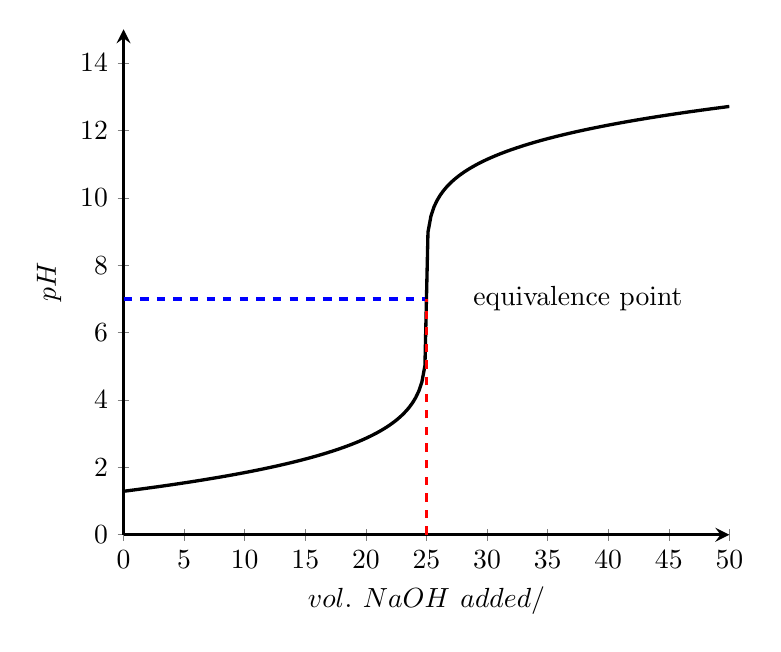
\begin{tikzpicture}

				\begin{axis}[
					axis lines		= left,
					domain			= 0:50,
					xlabel			= \textbf{$vol.\ NaOH\ added/\si{\cubic\centi\metre}$},
					ylabel			= \textbf{$pH$},
					axis line style	= very thick,
					height			= 80mm,
					samples			= 200,
					xtick			= {0, 5, 10, 15, 20, 25, 30, 35, 40, 45, 50}
				]

					\addplot[color = black, very thick, y filter/.code={\pgfmathparse{\pgfmathresult+7}}]{
						3 * ((x - 25)/abs(x - 25) * abs(x - 25)^(1/5))
					};

					% force the graph to show up to these
					\addplot[color = green, very thick, opacity = 0]{15};
					\addplot[color = green, very thick, opacity = 0]{0};

					\addplot[color = red, very thick, dashed] coordinates {(25, 0) (25, 7)};
					\addplot[color = blue, very thick, dashed, restrict x to domain = 0:25]{7};

					\node at (axis cs: 37.5,7) {equivalence point};

				\end{axis}

			\end{tikzpicture}
			\end{center}

			\begin{bulletlist}
				\ListProperties(Space*=-0.5em, Space=-0.5em)
				& $V = \SI{0}{\cubic\centi\metre}$
					\tabto{25mm}$pH = [acid]$, since only the strong acid exists.

				& $V < \SI{25}{\cubic\centi\metre}$
					\tabto{25mm}$pH < 7$, but increases, as more acid is neutralised.
					\tabto{25mm}No salt hydrolysis or buffer, since there is no weak acid or base.

				& $V = \SI{25}{\cubic\centi\metre}$
					\tabto{25mm}$pH = 7$, at the equivalence point.
					\tabto{25mm}No \ch{H+} or \ch{OH-} is present, so the solution is neutral.

				& $V > \SI{25}{\cubic\centi\metre}$
					\tabto{25mm}$pH > 7$, as [\ch{OH-}] increases due to the addition of more \ch{NaOH}.

			\end{bulletlist}

			\itl{Phenolphthalein}, \itl{methyl orange} or \itl{thymol blue} can be used as indicators. Of note is the sharp \pH{}
			change at the equivalence point in the titration curve.

		%end subsection
















		\pagebreak
		\subsection{Strong Acid, Weak Base}

			Here, the titration of \ch{H\Cl} against \ch{NH3}.

			\begin{center}
			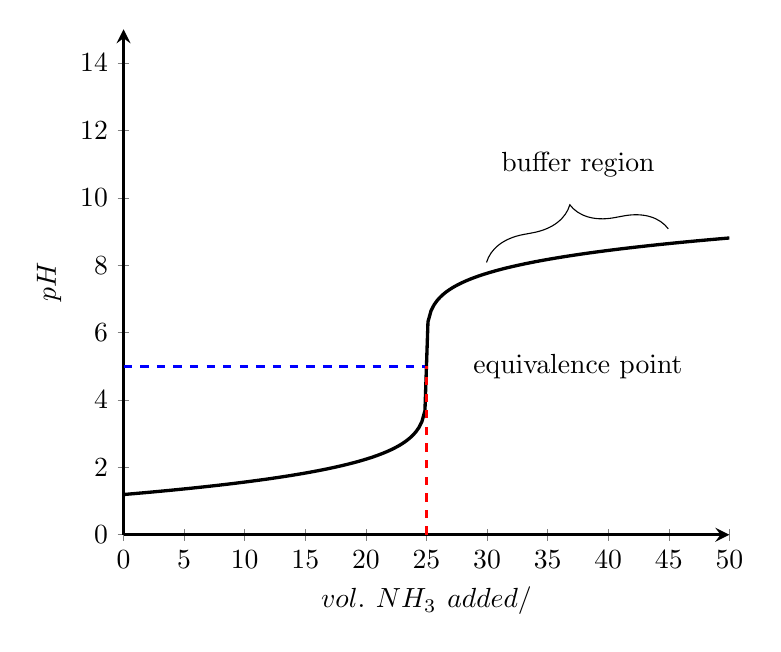
\begin{tikzpicture}

				\begin{axis}[
					axis lines		= left,
					domain			= 0:50,
					xlabel			= \textbf{$vol.\ NH_{3}\ added/\si{\cubic\centi\metre}$},
					ylabel			= \textbf{$pH$},
					axis line style	= very thick,
					height			= 80mm,
					samples			= 200,
					xtick			= {0, 5, 10, 15, 20, 25, 30, 35, 40, 45, 50}
				]

					\addplot[color = black, very thick, y filter/.code={\pgfmathparse{\pgfmathresult+5}}]{
						2 * ((x - 25)/abs(x - 25) * abs(x - 25)^(1/5))
					};

					% force the graph to show up to these
					\addplot[color = green, very thick, opacity = 0]{15};
					\addplot[color = green, very thick, opacity = 0]{0};

					\addplot[color = red, very thick, dashed] coordinates {(25, 0) (25, 5)};
					\addplot[color = blue, very thick, dashed, restrict x to domain = 0:25]{5};

					\node at (axis cs: 37.5,5) {equivalence point};

					\draw[decorate, decoration={brace,amplitude=15pt,raise=1pt}] (30,8) -- (45,9);
					\node at (axis cs: 37.5,11) {buffer region};

				\end{axis}

			\end{tikzpicture}
			\end{center}

			\begin{bulletlist}
				\ListProperties(Space*=-0.5em, Space=-0.5em)
				& $V = \SI{0}{\cubic\centi\metre}$
					\tabto{25mm}$pH = [acid]$, since only the strong acid exists.

				& $V < \SI{25}{\cubic\centi\metre}$
					\tabto{25mm}$pH < 7$, but increases, as more acid is neutralised.
					\tabto{25mm}No salt hydrolysis or buffer, since there is no weak acid or base.

				& $V = \SI{25}{\cubic\centi\metre}$
					\tabto{25mm}$pH < 7$, at the equivalence point.
					\tabto{25mm}Even though no \ch{H+} or \ch{OH-} is present, \ch{NH4+} in the salt hydrolyses,
					\tabto{25mm}forming acid: \ch{NH4+ + H2O >=< NH3 + H3O+}.

				& $V > \SI{25}{\cubic\centi\metre}$
					\tabto{25mm}$pH > 7$, as [\ch{OH-}] increases due to the addition of more base.
					\tabto{25mm}A buffer forms, since there is \ch{NH3} and its conjugate acid \ch{NH4+}.

			\end{bulletlist}

			\itl{Methyl orange} can be used as the indicator, since its working range is within the sharp \pH{} change.

		% end subsection



















		\pagebreak
		\subsection{Weak Acid, Strong Base}

			Here, the titration of \ch{CH3CO2H} against \ch{NaOH}.

			\begin{center}
			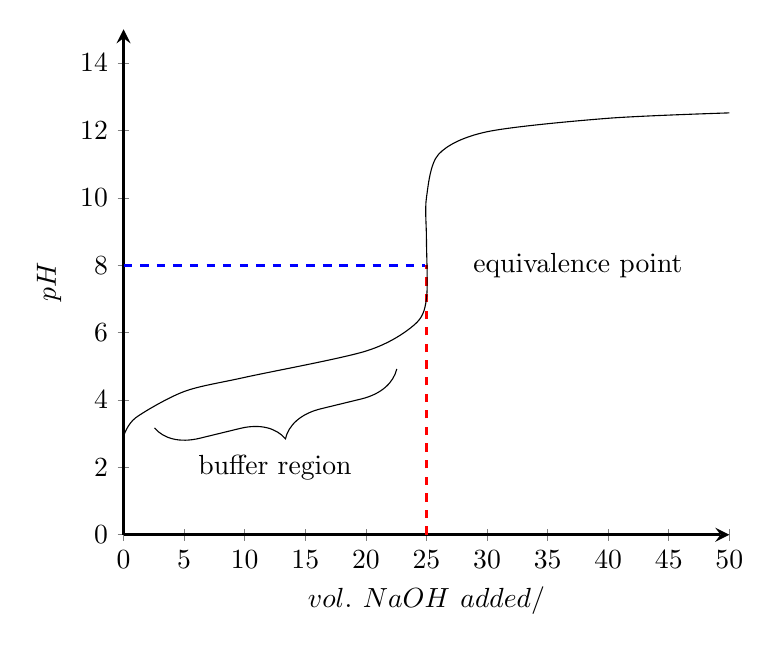
\begin{tikzpicture}

				\begin{axis}[
					axis lines		= left,
					domain			= 0:50,
					xlabel			= \textbf{$vol.\ NaOH\ added/\si{\cubic\centi\metre}$},
					ylabel			= \textbf{$pH$},
					axis line style	= very thick,
					height			= 80mm,
					samples			= 200,
					xtick			= {0, 5, 10, 15, 20, 25, 30, 35, 40, 45, 50}
				]

					% force the graph to show up to these
					\addplot[color = green, very thick, opacity = 0]{15};
					\addplot[color = green, very thick, opacity = 0]{0};

					\addplot[color = red, very thick, dashed] coordinates {(25, 0) (25, 8.0)};
					\addplot[color = blue, very thick, dashed, restrict x to domain = 0:25]{8.0};

					\node at (axis cs: 37.5,8) {equivalence point};

					\draw[decorate, decoration={brace,amplitude=15pt,raise=1pt,mirror}] (2.5,3.25) -- (22.5,5);
					\node at (axis cs: 12.5,2) {buffer region};



					% ORIGINAL DATASET:
					% (0,2.92) (1,3.47) (2,3.79) (3,3.98) (4,4.13) (5,4.25) (10,4.67) (15,5.03) (20,5.45) (21,5.57) (22,5.72)
					% (23,5.91) (24,6.23) (25,7.0) (25,8.78) (25,10.0) (26,11.29) (27,11.59) (28,11.75) (29,11.87) (30,11.96)
					% (35,12.22) (40,12.36) (45,12.46) (50,12.52)

					\addplot [color = black, mark = none, smooth] coordinates {
						(0,2.92) (1,3.47) (5,4.25) (10,4.67) (20,5.45) (24,6.23)
						(25,7.0) (25,8.78) (25,10.0) (26,11.29) (30,11.96) (40,12.36) (50,12.52)
					};

				\end{axis}

			\end{tikzpicture}
			\end{center}

			\begin{bulletlist}
				\ListProperties(Space*=-0.5em, Space=-0.5em)
				& $V = \SI{0}{\cubic\centi\metre}$
					\tabto{25mm}$pH > [acid]$, since the acid is weak.

				& $V < \SI{25}{\cubic\centi\metre}$
					\tabto{25mm}$pH < 7$, but increases, as more acid is neutralised.
					\tabto{25mm}A buffer forms; there is \ch{CH3CO2H} and its conjugate base \ch{CH3CO2-}.

				& $V = \SI{25}{\cubic\centi\metre}$
					\tabto{25mm}$pH > 7$, at the equivalence point.
					\tabto{25mm}Even though no \ch{H+} or \ch{OH-} is present, \ch{CH3CO2-} in the salt hydrolyses,
					\tabto{25mm}forming base: \ch{CH3CO2- + H2O >=< CH3CO2H + OH-}.

				& $V > \SI{25}{\cubic\centi\metre}$
					\tabto{25mm}$pH > 7$, as [\ch{OH-}] increases due to the addition of more base.
					\tabto{25mm}No buffer; there is no \ch{CH3CO2H} left, only its conjugate \ch{CH3CO2-}.


			\end{bulletlist}

			\itl{Phenolphthalein} or \itl{thymol blue} can be used as the indicator, since their working range lie within the sharp
			\pH{} change.

		% end subsection






















		\pagebreak
		\subsection{Weak Acid, Weak Base}

			Here, the titration of \ch{CH3CO2H} against \ch{NH3}.

			\begin{center}
			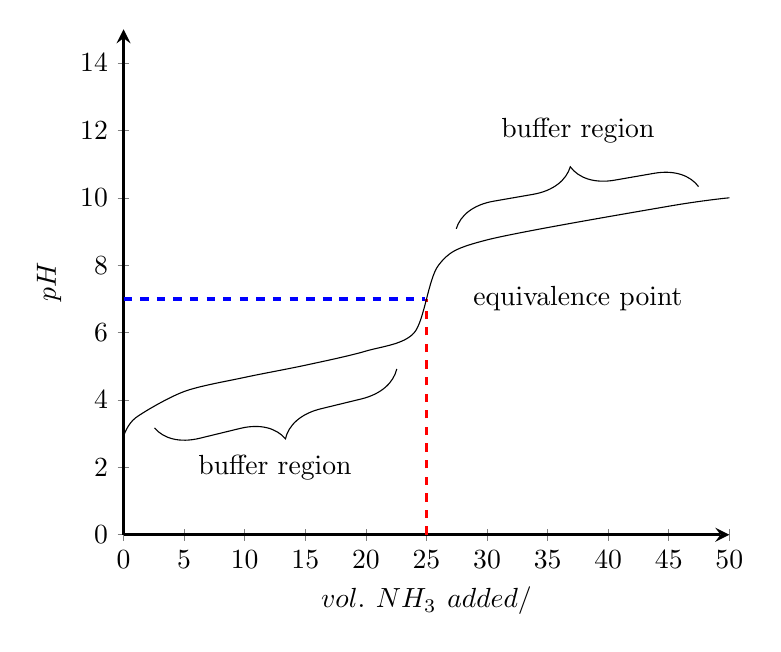
\begin{tikzpicture}

				\begin{axis}[
					axis lines		= left,
					domain			= 0:50,
					xlabel			= \textbf{$vol.\ NH_{3}\ added/\si{\cubic\centi\metre}$},
					ylabel			= \textbf{$pH$},
					axis line style	= very thick,
					height			= 80mm,
					samples			= 200,
					xtick			= {0, 5, 10, 15, 20, 25, 30, 35, 40, 45, 50}
				]

					% force the graph to show up to these
					\addplot[color = green, very thick, opacity = 0]{15};
					\addplot[color = green, very thick, opacity = 0]{0};

					\addplot[color = red, very thick, dashed] coordinates {(25, 0) (25, 7.0)};
					\addplot[color = blue, very thick, dashed, restrict x to domain = 0:25]{7.0};

					\node at (axis cs: 37.5,7) {equivalence point};

					\draw[decorate, decoration={brace,amplitude=15pt,raise=1pt,mirror}] (2.5,3.25) -- (22.5,5);
					\node at (axis cs: 12.5,2) {buffer region};

					\draw[decorate, decoration={brace,amplitude=15pt,raise=1pt}] (27.5,9.0) -- (47.5,10.25);
					\node at (axis cs: 37.5,12) {buffer region};

					\addplot [color = black, mark = none, smooth] coordinates {
						(0,2.92) (1,3.47) (5,4.25) (10,4.67) (15,5.03) (20,5.45)
						(24,6.0) (26,8.0) (30,8.75) (45,9.75) (50,10)
					};

				\end{axis}

			\end{tikzpicture}
			\end{center}

			\begin{bulletlist}
				\ListProperties(Space*=-0.5em, Space=-0.5em)
				& $V = \SI{0}{\cubic\centi\metre}$
					\tabto{25mm}$pH > [acid]$, since the acid is weak.

				& $V < \SI{25}{\cubic\centi\metre}$
					\tabto{25mm}$pH < 7$, but increases, as more acid is neutralised.
					\tabto{25mm}A buffer forms; there is \ch{CH3CO2H} and its conjugate base \ch{CH3CO2-}.

				& $V = \SI{25}{\cubic\centi\metre}$
					\tabto{25mm}$pH \approx 7$, at the equivalence point.
					\tabto{25mm}Both the conjugate base and conjugate acid hydrolyse:
					\tabto{25mm}\ch{CH3CO2- + H2O >=< CH3CO2H + OH-}
					\tabto{25mm}\ch{NH4+ + H2O >=< NH3 + H3O+}
					\tabto{25mm}The exact \pH{} depends on the \Ka{} and \Kb{} values of the conjugates.

				& $V > \SI{25}{\cubic\centi\metre}$
					\tabto{25mm}$pH > 7$, as [\ch{OH-}] increases due to the addition of more base.
					\tabto{25mm}A buffer forms; there is \ch{NH3} and its conjugate acid \ch{NH4+}.

			\end{bulletlist}

			No suitable indicator can be used, since there is no sharp \pH{} change at all. A \pH{} meter can be used instead. Note that
			the \pH{} at the equivalence point is not necessarily \num{7} --- following the situation of simultaneous salt hydrolysis of
			a weak acid and base:

			\begin{bulletlist}
				& $K_{a} > K_{b}$;\hspace{4mm} $[H_{3}O^{+}] > [OH^{-}]$;\hspace{4mm} acidic solution
				& $K_{a} = K_{b}$;\hspace{4mm} $[H_{3}O^{+}] = [OH^{-}]$;\hspace{4mm} neutral solution
				& $K_{a} < K_{b}$;\hspace{4mm} $[H_{3}O^{+}] < [OH^{-}]$;\hspace{4mm} basic solution
			\end{bulletlist}

			In this case, the \Ka{} and \Kb{} of \ch{NH3+} and \ch{CH3CO2H} are almost equal (\SI{1.8e-5}{\molarConc}), so
			the \Kb{} and \Ka{} of their conjugates will be as well.


		% end subsection










		\pagebreak
		\subsection{Titration of Polyprotic Acids or Bases}

			Polyprotic acids are acids with multiple ionisable protons; conversely polybasic bases are those that can accept more than one
			proton.

			\ch{H2CO3} is a polyprotic acid with a weak second acid \ch{HCO3-}, while \ch{H2SO4} is a strong polyprotic acid with a strong
			first acid and a weak second acid \ch{HSO4-}. Often times the \Ka{} of the first proton is much larger than that of subsequent ones.

			When analysing polyprotic things, it is often convenient and apt to assume that every molecule of acid will first lose one proton,
			before starting to lose the second.

			Thus, a distinct titration curve can be seen, in this case using the example of \ch{CO3^2-}, which is the conjugate base of
			the weak acid polyprotic \ch{H2CO3}:

			\txtdiagram{
				\schemestart[0,1.0,thick]
					\ch{CO3^2- \stAq}\hspace{2mm} + \hspace{2mm}\ch{H+ \stAq}
					\arrow\ch{HCO3- \stAq}
					\arrow(@c1.south east--.north east){0}[-90,.15]
					\ch{HCO3- \stAq}\hspace{2mm} + \hspace{2mm}\ch{H+ \stAq}
					\arrow\ch{H2CO3 \stAq}
				\schemestop
			}{\vspace{-2em}}


			\begin{center}
			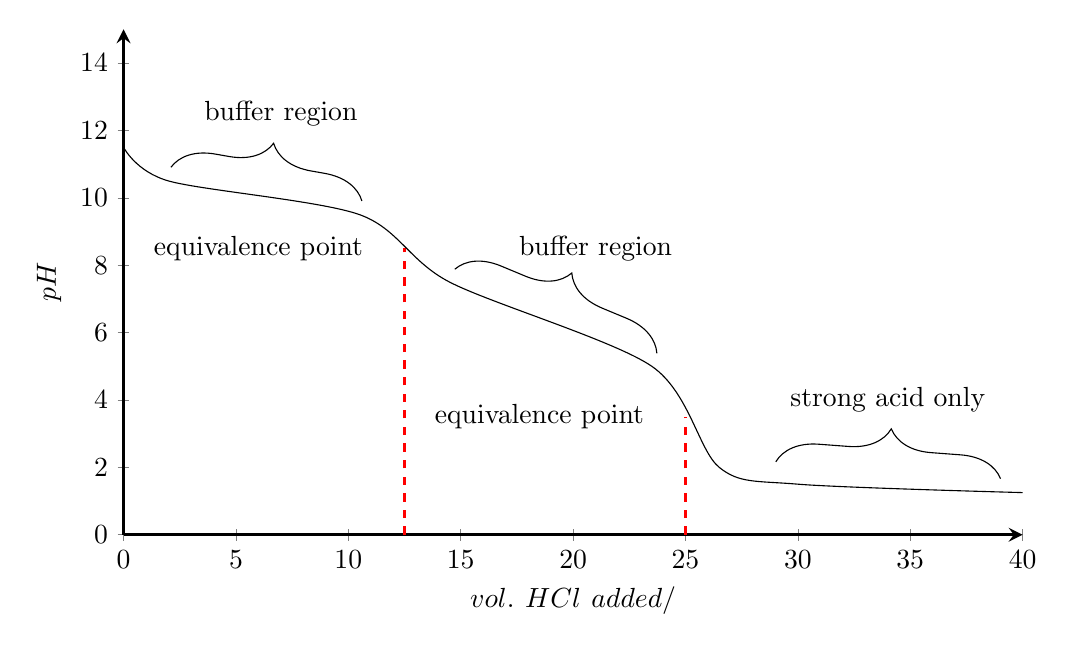
\begin{tikzpicture}

				\begin{axis}[
					axis lines		= left,
					domain			= 0:40,
					xlabel			= \textbf{$vol.\ HCl\ added/\si{\cubic\centi\metre}$},
					ylabel			= \textbf{$pH$},
					axis line style	= very thick,
					height			= 80mm,
					width			= 130mm,
					samples			= 200,
					xtick			= {0, 5, 10, 15, 20, 25, 30, 35, 40}
				]

					% force the graph to show up to these
					\addplot[color = green, very thick, opacity = 0]{15};
					\addplot[color = green, very thick, opacity = 0]{0};

					\addplot[color = red, very thick, dashed] coordinates {(12.5, 0) (12.5, 8.5)};
					\addplot[color = red, very thick, dashed] coordinates {(25, 0) (25, 3.5)};


					\node at (axis cs: 6,8.5) {equivalence point};
					\node at (axis cs: 18.5,3.5) {equivalence point};

					\draw[decorate, decoration={brace,amplitude=15pt,raise=5pt}] (2,10.5) -- (10.5,9.5);
					\node at (axis cs: 7,12.5) {buffer region};

					\draw[decorate, decoration={brace,amplitude=15pt,raise=5pt}] (14.5,7.5) -- (23.5,5.0);
					\node at (axis cs: 21,8.5) {buffer region};

					\draw[decorate, decoration={brace,amplitude=15pt,raise=2pt}] (29,2.0) -- (39,1.5);
					\node at (axis cs: 34,4) {strong acid only};

					\addplot [color = black, smooth] coordinates {
						(0, 11.5) (2, 10.5) (10.5, 9.5) (14.5, 7.5)
						(23.5, 5.0) (26.5, 2.0) (30, 1.5) (40, 1.25)
					};

				\end{axis}

			\end{tikzpicture}
			\end{center}

			There are two distinct equivalence points here, and they should be observed separately with two indicators ---
			\itl{phenolphthalein} for the first equivalence point at $pH = 8.5$, and \itl{methyl orange} for the second one
			at $pH = 3.5$.

			\itl{Methyl orange} should only be added to the solution after the first equivalence point is observed, if not the first
			point will be obscured since methyl orange exhibits no colour change at that point.


		% end subsection

	% end section







	\section{\MpH{} Indicators}

		\subsection{Working Range}

			Indicators exist in an equilibrium with \ch{H+}; the colour of the indicator depends on the ratio of the concentration of
			one ion to the other. For instance, taking an arbitrary indicator species \ch{In-} and its conjugate \ch{HIn}:

			\txtdiagram{
				\schemestart[0,1.0,thick]
					\ch{In- \stAq}\hspace{2mm} + \hspace{2mm}\ch{H+ \stAq}
					\arrow{<=>}
					\ch{HIn \stAq}
				\schemestop
			}{\vspace{-2em}}

			Following the general formula for \Ka{}, and manipulating slightly:

			\diagram[1.5]{
				$K_{In} = \frac{[H^{+}][In^{-}]}{[HIn]}$
				\hspace{15mm}
				$pH = pK_{In} + lg(\frac{[In^{-}]}{[HIn]})$
			}{\vspace{-1.5em}}

			For the colour change to be visible, the concentration of the dominant ion must be greater than the less dominant one
			by a factor of 10, so the working range of an indicator is as such:

			\diagram[1.5]{
				$pH = pK_{In} ± 1$
			}{\vspace{-1.5em}}

		% end subsection



		\pagebreak
		\subsection{Appropriate Indicator Selection}

			When selecting which indicator to use, the most obvious consideration is that the colour change will occur at the equivalence
			point of the reaction --- if not it is pointless. For any indicator to be used at all, there should be a sharp change at said
			equivalence point; titrations involving at least one \itl{strong} acid or base (or both) will exhibit such a sharp change.

			The working \pH{} ranges for a number of common indicators, and their uses, are summarised below:


			\begin{center}\begin{table}[htb]\renewcommand{\arraystretch}{1.5}
			\begin{tabu} to \textwidth {| X[c,m] | X[c,m] | X[c,m] |}

				\hline
				% headings
				Indicator		& 	Working Range (\pH{})	& 	Colour (Low/High)	\\	\hline

				Methyl Orange	&	\numrange{3.1}{4.4}		&	Red / Yellow		\\	\hline
				Phenolphthalein	&	\numrange{8.0}{9.6}		&	Colourless / Pink	\\	\hline
				Thymol Blue		&	\numrange{8.0}{9.6}		&	Yellow / Blue		\\	\hline


			\end{tabu}
			\end{table}\end{center}\vspace{-10mm}

			Next, according to their working \pH{} ranges, a summary of the suitable indicators for each kind of titration:


			\begin{center}\begin{table}[htb]\renewcommand{\arraystretch}{1.5}
			\newcolumntype{M}[1]{>{\centering\arraybackslash}m{#1}}
			\begin{tabu} to \textwidth {| M{50mm} | M{35mm} | X[c,m] |}
			%| X[c,m] | X[c,m] | X[c,m] |}

				\hline
				% headings
				Situation					& 	Sharp \pH{} Change		& 	Indicators						\\	\hline
				Strong Acid, Strong Base	&	\numrange{3.0}{11.0}	&	Any								\\	\hline
				Strong Acid, Weak Base		&	\numrange{3.0}{7.0}		&	Methyl Orange					\\	\hline
				Weak Acid, Strong Base		&	\numrange{7.0}{11.0}	&	Phenolphthalein, Thymol Blue	\\	\hline
				Weak Acid, Weak Base		&	\itl{none}			&	\itl{none}					\\	\hline


			\end{tabu}
			\end{table}\end{center}\vspace{-10mm}

		% end subsection

	% end section

% end part































